\chapter{أشكال الطاقة وتحويلاتها}\label{ch:g9:energy-conversions}

جرت \omterm{def:g5:everyday-energy:energy}{الطاقة} في هذا الكتاب كنهر تحت مدينة --- تُلمَح عند كل زاوية،
ولم تُرسَم خريطتها كاملة قطّ. وقد آن الأوان. فينال كل شكل
اسمه، وينال أحدها صيغة هذه السنة العظيمة الثانية، ويترأّسها
جميعًا أعظم قانون محاسبة في العلم: المجموع لا يتغيّر أبدًا.
البتّة.

\section{الأشكال، مجموعةً}

\begin{definition}[أشكال الطاقة]\label{def:g9:energy-conversions:forms}
أشكال \omterm{def:g5:everyday-energy:energy}{الطاقة}، معروضةً رسميًّا: \emph{\omterm{prop:g9:kinetic-energy-safety:formula}{الطاقة الحركية}} --- حصة
الحركة، $\frac12 m v^2$؛ و\emph{الطاقة الكامنة}\index{طاقة
كامنة} --- مخزونة بالموضع أو بالترتيب (المرفوع، والممدود،
والمضغوط)؛ و\emph{\omterm{def:g5:everyday-energy:energy}{الطاقة} الحرارية} --- \omterm{def:g3:sound-around-us:vibration}{الاهتزاز} الجزيئي
الفوضوي الذي تقيسه \omterm{def:g3:temperature-thermometers:temperature}{درجة الحرارة}؛ و\emph{\omterm{def:g5:everyday-energy:energy}{الطاقة} الكيميائية} ---
مخزونة في ترتيبات المادة: الغذاء والوقود والبطاريات؛
و\emph{\omterm{def:g5:everyday-energy:energy}{الطاقة} الكهربائية} --- ما يسلّمه التيار السائر؛
و\emph{\omterm{def:g5:everyday-energy:energy}{الطاقة} الإشعاعية} --- يحملها \omterm{def:g1:light-and-shadows:source}{الضوء} نفسه، وهي صورة شحن
\omterm{def:g1:light-and-shadows:source}{ضوء} الشمس؛ و\emph{\omterm{def:g5:everyday-energy:energy}{الطاقة} النووية} --- محبوسة في لبّ الذرّة،
وهي أعمق مخزون فتحه البشر.
\end{definition}

\begin{proposition}[الطاقة الكامنة الثقالية]\label{prop:g9:energy-conversions:ep}
رفع \omterm{def:g3:measuring-mass:mass}{كتلة} $m$ (\omterm{def:g6:measurement-in-science:measuring}{بوحدة} \unit{kg}) إلى ارتفاع $h$ (\omterm{def:g6:measurement-in-science:measuring}{بوحدة}
\unit{m}) في مواجهة $g$ \omterm{def:g9:gravitation:gravitation}{الجاذبية} يخزن فيها \omterm{def:g9:energy-conversions:forms}{الطاقة الكامنة}
\[
E_p = m \times g \times h
\]
\omterm{def:g9:kinetic-energy-safety:joule}{بالجول} --- قابلةً للاسترجاع كاملةً في طريق النزول. فالفأس
المرفوع، والأرجوحة المسحوبة إلى الخلف، والبحيرة الجبلية: كلها
تملك $m g h$ في الحساب. (وهي الصيغة المستعارة في ملصقات سلامة
الطرق --- وقد صارت رسميًّا لك.)
\end{proposition}

\begin{example}[المبادلة الكبرى: $E_p$ في مقابل $E_k$]\label{ex:g9:energy-conversions:trade}
أسقط كرة من ارتفاع $h$: يتحوّل حسابها، وهي تسقط، جولًا \omterm{def:g9:kinetic-energy-safety:joule}{بجول}،
من الكامنة إلى الحركية. وعند الأرض يكون $m g h$ كله قد صار
$\frac12 m v^2$ --- ساوِ بينهما تُختصر \omterm{def:g3:measuring-mass:mass}{الكتلة}:
\[
v = \sqrt{2 g h},
\]
فيكسب جذر هذه السنة التربيعي قوته. فمن \qty{20}{m}:
$v = \sqrt{2 \times 9.8 \times 20} \approx \qty{20}{m/s}$ ---
أي سبعون كيلومترًا في الساعة، مهما تكن \omterm{def:g3:measuring-mass:mass}{الكتلة}. والبندول يلعب
المبادلة في الاتجاهين إلى الأبد (ناقص همسة \omterm{def:g2:air-around-us:air}{للهواء})؛ ومتزلّج
نصف الأنبوب كذلك: ارتفاع \omterm{def:g7:motion-average-speed:formula}{فسرعة} فارتفاع، والصيغتان تمرّران
مجموعًا واحدًا ذهابًا وإيابًا.
\end{example}

\begin{omfigure}
\begin{tikzpicture}[scale=0.8]
  \draw[very thick, omExo]
    (0.4,3.4) .. controls (2.2,0.2) and (4.2,0.2) .. (6.0,3.0)
    .. controls (7.0,4.6) and (8.4,4.6) .. (9.6,3.2);
  \fill[omDef] (0.4,3.4) circle (0.16);
  \fill[omDef] (3.2,0.62) circle (0.16);
  \fill[omDef] (7.2,4.15) circle (0.16);
  \node[above, font=\footnotesize, align=center] at (0.9,3.6)
    {كلها $E_p$،\\ولا سرعة};
  \node[below, font=\footnotesize, align=center] at (3.2,0.4)
    {كلها $E_k$:\\أسرع ما يكون هنا};
  \node[above, font=\footnotesize, align=center] at (7.2,4.35)
    {مبادلة عائدة:\\بطيء عند القمّة};
\end{tikzpicture}

{\small دفتر الأفعوانية: الارتفاع المنفَق يشتري \omterm{def:g7:motion-average-speed:formula}{سرعة}، \omterm{def:g7:motion-average-speed:formula}{والسرعة}
المنفَقة تشتري الارتفاع ثانية --- مجموع واحد، وحسابان، والمجموع
راكب بلا تغيّر (إلا ما يقشطه الاحتكاك في هدوء).}
\end{omfigure}

\section{القانون العظيم}

\begin{proposition}[انحفاظ الطاقة]\label{prop:g9:energy-conversions:conservation}
في كل عملية فُحصت يومًا --- التصادمات والكيمياء، والآلات
والعواصف، والنجوم والخلايا --- تغيّر \omterm{def:g5:everyday-energy:energy}{الطاقة} شكلها ومالكها،
لكن \emph{المجموع} ينحفظ بالضبط: فلا شيء يُخلق، ولا شيء يفنى،
وكل \omterm{def:g9:kinetic-energy-safety:joule}{جول} محسوب. وهذا أعمق قانون محاسبة في الفيزياء: به تقاعدت
آلات الأبد في فصول الطفولة، وبه تُدقَّق كل سلسلة في هذا
الكتاب، ولم تضبطه تجربة واحدة في ثلاثة قرون على خطأ. (وأمّا
لماذا تحفظ الطبيعة هذا القانون بكل هذا الوفاء فسؤال عميق له
جواب جميل --- من جواهر سنوات الجامعة.)
\end{proposition}

\begin{method}[تدقيق أيّ عملية]\label{met:g9:energy-conversions:audit}
محاسبة الفيزيائي الكونية:
\begin{enumerate}
  \item سيّج الجملة --- ما الداخل في التدقيق؛
  \item اسرد حسابات \omterm{def:g5:everyday-energy:energy}{الطاقة} قبل: كل شكل، وكل مخزون؛
  \item واسردها بعد --- بما في ذلك، دائمًا، الفكّة الحرارية:
        دفء الاحتكاك، وهمسة \omterm{def:g3:sound-around-us:sound}{الصوت}؛
  \item ووازن الدفاتر: يجب أن يتطابق المجموعان. والعجز يعني
        أن شكلًا لم يُحصَ --- فابحث ثانية عن التسرّب؛ وهو
        دافئ عادةً.
\end{enumerate}
\end{method}

\begin{example}[تدقيقات محلولة]\label{ex:g9:energy-conversions:audits}
السيارة الكابحة: الحساب الحركي مفرَّغ، والحساب الحراري عند
الأقراص مقيَّد بالكامل --- تقاعد لا إفناء. والكرة النطّاطة التي
تخبو: كل نطّة تقشط من الحركية إلى دفء الكرة والأرض؛ جواب
الطفولة، وقد صار قابلًا للتدقيق. وفطورك وأنت تصعد التلّة على
درّاجة: المخزون الكيميائي هابطًا، والحساب الكامن صاعدًا ($m g h$
لك وللدرّاجة)، والحصة الحرارية مشعَّة --- فالعضلات تعمل دافئة.
وكل لغز من ألغاز فصول \omterm{def:g5:everyday-energy:energy}{الطاقة} الباكرة ينغلق تحت الأعمدة الثلاثة
نفسها.
\end{example}

\section{المردود}

\begin{definition}[المردود]\label{def:g9:energy-conversions:efficiency}
\emph{مردود}\index{مردود} محوِّل هو الجزء من طاقته الداخلة
المسلَّم في الشكل المطلوب:
\[
\text{المردود} =
\frac{\text{الطاقة النافعة الخارجة}}{\text{الطاقة الكلّية الداخلة}},
\]
وهو عدد بين $0$ و$1$ (أو نسبته المئوية). والباقي لا يفنى ---
فالانحفاظ يمنع --- بل يهرب في أشكال غير مطلوبة، وهي الدفء في
كل الأحوال تقريبًا.
\end{definition}

\begin{example}[بطاقات تقدير]\label{ex:g9:energy-conversions:reportcards}
\omterm{def:g3:first-electric-circuit:bulb}{المصباح} السلف المتوهّج: خمسة في المئة \omterm{def:g1:light-and-shadows:source}{ضوء}، وخمسة وتسعون
دفئًا --- مسخّن ذو هواية. وخلفه الحديث: ثلاثون في المئة وزيادة،
والباقي دفء أيضًا. ومحرّك سيارة: نحو الثلث حركة نافعة، والثلثان
إلى المشعّ والعادم. \omterm{ex:g6:circuits-and-safety:motor}{والمحرّك} الكهربائي: فوق التسعين. والمولّدات
المتناوبة العظيمة: قرب التسعة والتسعين --- أفضل محوّلات
الحضارة. ولا يبلغ محوّل أمين المئة: فبعض التسرّب إلى الدفء
عمولة الطبيعة الكونية.
\end{example}

\begin{omfigure}
\begin{tikzpicture}[scale=0.8]
  \draw[omDef, fill=omDef, fill opacity=0.4]
    (0.3,1.2) rectangle (4.2,2.6);
  \node[font=\small] at (2.25,1.9) {الداخل: \qty{100}{J}};
  \draw[omMeth, fill=omMeth, fill opacity=0.4]
    (7.4,2.0) rectangle (11.2,2.9);
  \node[font=\footnotesize] at (9.3,2.45)
    {النافع: \qty{35}{J}};
  \draw[omThm, fill=omThm, fill opacity=0.35]
    (7.4,0.6) rectangle (11.2,1.75);
  \node[font=\footnotesize] at (9.3,1.17)
    {الدفء: \qty{65}{J}};
  \draw[-Stealth, very thick] (4.3,2.25) -- (7.3,2.5);
  \draw[-Stealth, very thick] (4.3,1.55) -- (7.3,1.2);
  \node[above, font=\small] at (5.8,2.65) {محوِّل};
\end{tikzpicture}

{\small مخطّط \omterm{def:g9:energy-conversions:efficiency}{مردود}: مئة \omterm{def:g9:kinetic-energy-safety:joule}{جول} داخلة، وخمسة وثلاثون مسلَّمة كما
يُراد، وخمسة وستّون متسرّبة دفئًا --- ولا \omterm{def:g9:kinetic-energy-safety:joule}{جول} واحد ناقص من
المجموع.}
\end{omfigure}

\begin{omfigure}
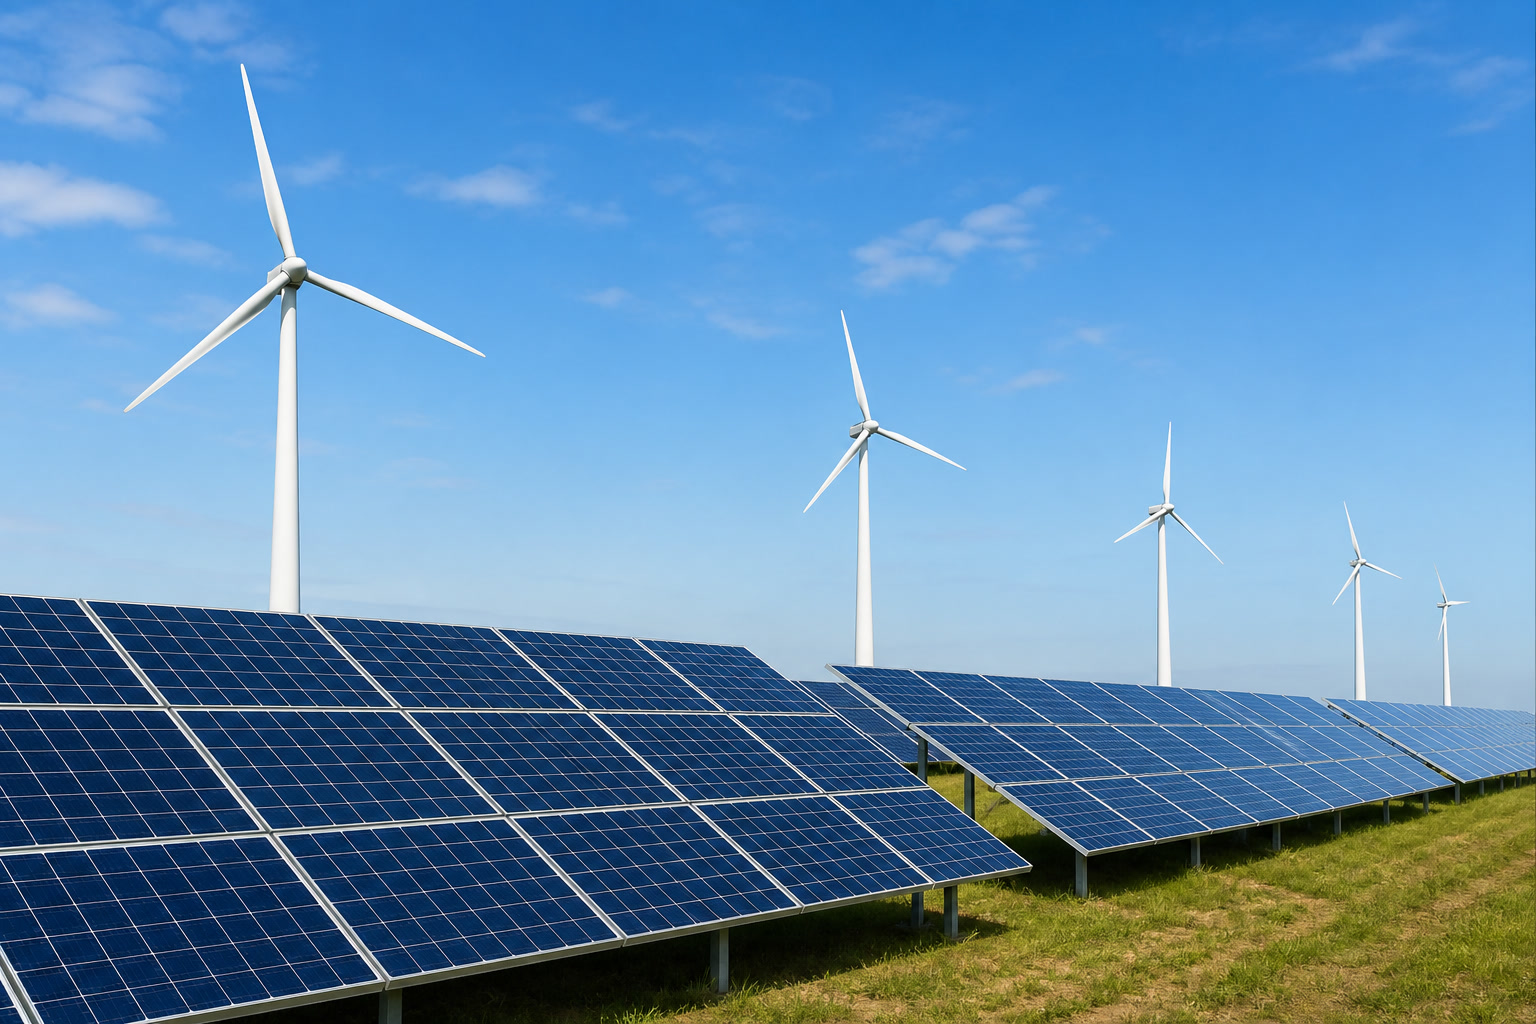
\includegraphics[width=0.55\linewidth]{images/book1/ai/g9-energy-solar-wind.jpg}

{\small محوّلان في حقل واحد: \omterm{def:g1:light-and-shadows:source}{ضوء} الشمس إلى \omterm{def:g5:everyday-energy:energy}{طاقة} كهربائية في الألواح، \omterm{def:g2:air-around-us:air}{وهواء} متحرّك إلى \omterm{def:g5:everyday-energy:energy}{طاقة} كهربائية في العنفات.}
\end{omfigure}

\begin{remark}[ماذا يعني ``توفير الطاقة'' حقًّا]\label{rem:g9:energy-conversions:saving}
إن كان الانحفاظ يحرس كل \omterm{def:g9:kinetic-energy-safety:joule}{جول}، فلماذا على أحد أن ``يوفّر
\omterm{def:g5:everyday-energy:energy}{الطاقة}''؟ لأن القانون يحفظ \emph{المقدار}، لا \emph{النفع}.
فالمخزونات المركَّزة --- الوقود، والشحنة، والارتفاع --- يمكن
أن تُنفق إلى دفء منتشر رقيقًا في العالم، والدفء المنتشر، وإن
نجا كل \omterm{def:g9:kinetic-energy-safety:joule}{جول} منه، لم يعد يستطيع أن يسوق غلّايات ولا قطارات: فقد
جرى النهر إلى أسفل. ومشكلة الحضارة مع \omterm{def:g5:everyday-energy:energy}{الطاقة} ليست شحّ الجولات
--- فالشمس تغمرنا بآلاف أضعاف حاجتنا --- بل حسن تدبير
\emph{النافع} منها. وتلك الفكرة، مصوغةً بدقّة، من أشهر قصص
الفيزياء؛ وهي تنتظر في سنوات الجامعة باسمها الذائع.
\end{remark}

\section{تمارين}

\begin{exercise}[$\star$]\label{exo:g9:energy-conversions:1}
سمِّ أشكال الفهرس السبعة، ولكل واحد مثال منزلي.
\end{exercise}

\begin{exercise}[$\star$]\label{exo:g9:energy-conversions:2}
احسب $E_p$: دلو كتلته \qty{2}{kg} مرفوعًا \qty{10}{m}؛ ومتنزّه
كتلته \qty{60}{kg} على قمّة تسلّق \qty{500}{m}.
\end{exercise}

\begin{exercise}[$\star$]\label{exo:g9:energy-conversions:3}
اذكر قانون الانحفاظ، وماذا فعل بآلات الأبد في فصول طفولتك.
\end{exercise}

\begin{exercise}[$\star$]\label{exo:g9:energy-conversions:4}
دقّق البندول عبر أرجحة واحدة: الحسابات في الأعلى، وفي الأسفل،
والانجراف البطيء الإجمالي --- إلى أين؟
\end{exercise}

\begin{exercise}[$\star$]\label{exo:g9:energy-conversions:5}
استعمل $v = \sqrt{2 g h}$: \omterm{def:g7:motion-average-speed:formula}{سرعة} الارتطام من لوح غطس ارتفاعه
\qty{5}{m} --- ولماذا لم تدخل \omterm{def:g3:measuring-mass:mass}{كتلة} الغاطس أبدًا.
\end{exercise}

\begin{exercise}[$\star$]\label{exo:g9:energy-conversions:6}
عرّف \omterm{def:g9:energy-conversions:efficiency}{المردود}. محرّك يأخذ \qty{200}{J} ويسلّم \qty{170}{J} من
الحركة: ما \omterm{def:g9:energy-conversions:efficiency}{المردود}، وما مصير الباقي؟
\end{exercise}

\begin{exercise}[$\star$]\label{exo:g9:energy-conversions:7}
لماذا سُمّي \omterm{def:g3:first-electric-circuit:bulb}{المصباح} السلف بحقّ ``مسخّنًا ذا هواية''؟ أعطِ
النسبتين معًا.
\end{exercise}

\begin{exercise}[$\star$]\label{exo:g9:energy-conversions:8}
اكتب سلسلة التحويل الكاملة لصعود الدرّاج --- من الفطور إلى
القمّة --- مسمّيًا كل شكل وكل تسرّب.
\end{exercise}

\begin{exercise}[$\star\star$]\label{exo:g9:energy-conversions:9}
دفتر السدّ: \qty{1000}{kg} من الماء تسقط \qty{50}{m} عبر
العنفات. احسب $E_p$ المسلَّمة؛ وعند تحويل بتسعين في المئة،
\omterm{def:g5:everyday-energy:energy}{الطاقة} الكهربائية لكل طنّ --- والأطنان في الثانية اللازمة لخرج
\qty{4.4e6}{W}.
\end{exercise}

\begin{exercise}[$\star\star$]\label{exo:g9:energy-conversions:10}
كرة كتلتها \qty{0.5}{kg} تُسقط من \qty{2}{m} فترتدّ إلى
\qty{1.2}{m}. دقّق النطّة: الطاقتان قبل وبعد، \omterm{def:g6:mass-and-volume:volume}{وحجم} القشطة
ووجهتها --- وارتفاع الارتداد الذي لا يجد بعده أيّ تدقيق \omterm{prop:g9:kinetic-energy-safety:formula}{طاقة
حركية} ولا كامنة.
\end{exercise}

\begin{exercise}[$\star\star$]\label{exo:g9:energy-conversions:11}
``المصعد يحوّل \omterm{def:g5:everyday-energy:energy}{الطاقة} الكهربائية إلى \omterm{def:g9:energy-conversions:forms}{طاقة كامنة} \omterm{def:g9:energy-conversions:efficiency}{بمردود} تسعين
في المئة.'' احسب \omterm{def:g5:everyday-energy:energy}{الطاقة} الكهربائية اللازمة لرفع مقصورة كتلتها
\qty{500}{kg} مسافة \qty{30}{m} --- ووفّق بين العشرة في المئة
الزائدة وقانون الانحفاظ.
\end{exercise}

\begin{exercise}[$\star\star\star$]\label{exo:g9:energy-conversions:12}
متزلّج نصف الأنبوب ينطلق من السكون عند الحافة اليسرى، على
ارتفاع \qty{4}{m}. تنبّأ \omterm{def:g7:motion-average-speed:formula}{بسرعة} العبور في الأسفل، وبالارتفاع
المبلوغ على اليمين --- مثاليًّا وواقعيًّا --- وارسم المصير
الطويل الأمد للحركة ولطاقتها. ثم اشرح، بمقتضى
\cref{rem:g9:energy-conversions:saving}، لماذا لا يمكن أبدًا
استرجاع دفعة عند الحافة كاملةً: ماذا كسب دفتر العالم، وماذا
خسر المتزلّج بلا رجعة؟
\end{exercise}

\section{مسألة: لجنة مدينة الملاهي}

\begin{problem}[{مسألة نهاية الأسبوع --- مدينة الملاهي تستأجر
مستشار فيزياء؛ أفعوانيات وأبراج ودفتر لا يكذب}]\label{pb:g9:energy-conversions:1}
على ألعاب المدينة الجديدة أن تجتاز تدقيقك \omterm{def:g5:everyday-energy:energy}{للطاقة} قبل يوم
الافتتاح. خذ $g = \qty{9.8}{N/kg}$؛ وأهمِل الاحتكاك حتى يأبى
أن يُهمَل.

\medskip\noindent\textbf{القسم الأول --- الهبوط الكبير.}
قطار أفعوانية كتلته \qty{2000}{kg} يُرفع \omterm{def:g3:levers-and-scales:lever}{برافعة} إلى قمّة
\qty{45}{m} ويُطلق من السكون.
\begin{enumerate}
  \item ما $E_p$ للقطار عند القمّة؟
  \item وما سرعته المثالية في أسفل الهبوط، بالصيغة التي
        تختصر \omterm{def:g3:measuring-mass:mass}{الكتلة} --- بوحدتَي \unit{m/s} و\unit{km/h}؟
  \item ويضيف المصمّمون تلّة ثانية ارتفاعها \qty{50}{m} بعد
        الهبوط مباشرة. ارفضها بالدفتر --- واذكر أعلى تلّة
        ثانية يستطيع القطار المثالي أن يعلوها.
  \item \omterm{def:g7:motion-average-speed:formula}{والسرعة} المقيسة في الأسفل \qty{28}{m/s}، لا
        المثالية. احسب الطاقتين الحركيتين وقيّد الفرق في
        حسابه الصحيح.
\end{enumerate}

\medskip\noindent\textbf{القسم الثاني --- \omterm{def:g3:levers-and-scales:lever}{الرافعة}
والفاتورة.}
\begin{enumerate}[resume]
  \item ترفع \omterm{def:g3:levers-and-scales:lever}{الرافعة} القطار إلى قمّته في \qty{60}{s}. فما
        قدرتها عند \omterm{def:g9:energy-conversions:efficiency}{مردود} تامّ؟
  \item \omterm{def:g3:levers-and-scales:lever}{والرافعة} الحقيقية تسحب \qty{20}{kW}. فما مردودها؟
  \item وكل جولة تنطلق مرة كل أربع دقائق، عشر ساعات في
        اليوم. فما \omterm{def:g5:everyday-energy:energy}{طاقة} \omterm{def:g3:levers-and-scales:lever}{الرافعة} اليومية \omterm{def:g9:electric-power-energy:kwh}{بالكيلوواط ساعة}
        (\omterm{def:g3:levers-and-scales:lever}{بالرافعة} الحقيقية، وبعدّ الرفعات)، وما كلفتها عند
        $0.25$ \omterm{def:g6:measurement-in-science:measuring}{للوحدة}؟
  \item ويقترح مصمّم استرجاع \omterm{def:g5:everyday-energy:energy}{طاقة} وصول القطار بكابح مولِّد
        يغذّي الشبكة --- ``فتدفع اللعبة ثمن نفسها!'' دقّق
        الحلم: أيّ جزء يمكن أن يعود واقعيًّا، وأيّ قانون يمنع
        الدائرة الكاملة؟
\end{enumerate}

\medskip\noindent\textbf{القسم الثالث --- برج السقوط الحرّ
والتقرير.}
برج ارتفاعه \qty{60}{m} يُسقط مقصورة كتلتها \qty{500}{kg} إلى
مكابح مغناطيسية عند \qty{10}{m}.
\begin{enumerate}[resume]
  \item ما \omterm{def:g7:motion-average-speed:formula}{السرعة} عند دخول منطقة الكبح (بسقوط مثالي
        \qty{50}{m})؟
  \item وما \omterm{def:g5:everyday-energy:energy}{الطاقة} التي يجب أن تقاعدها المكابح، وإلى أين
        يرسلها التحريض؟ (فالمكابح أبناء عمومة لفصل \omterm{def:g9:alternator:alternator}{المولّد
        المتناوب} --- دوّامات من تيار محرَّض تسخّن المعدن.)
  \item ويصرخ الركّاب أنهم كانوا ``بلا \omterm{def:g4:weight-and-mass:weight}{وزن}'' أثناء السقوط.
        بمقتضى فكرة الرفقاء الساقطين في فصل \omterm{def:g9:gravitation:gravitation}{الجاذبية}، احكم في
        الزعم في جملة واحدة.
  \item وقّع تقرير اللجنة: ثلاث جمل --- المبادلة التي تحيا
        بها الأفعوانية، والقانون الذي أطاعته كل لعبة، والحساب
        الذي فرض عليها كلها ضريبة في هدوء.
\end{enumerate}
\end{problem}
